\documentclass[10pt,twocolumn]{article}
\usepackage[utf8]{inputenc}
\usepackage[T1]{fontenc}
\usepackage[margin=0.8in]{geometry}
\usepackage{booktabs}
\usepackage{multirow}
\usepackage{amsmath,amssymb}
\usepackage{graphicx}
\usepackage{xcolor}
\usepackage{authblk}
\usepackage{titlesec}
\usepackage{tikz}
\usetikzlibrary{arrows.meta,positioning,fit,backgrounds,calc,shapes.geometric}
\usepackage[hidelinks]{hyperref}
\titleformat{\section}{\normalfont\large\bfseries}{\thesection}{0.5em}{}
\titleformat{\subsection}{\normalfont\normalsize\bfseries}{\thesubsection}{0.5em}{}
\setlength{\parskip}{2pt}
\newcommand{\code}[1]{\texttt{\small #1}}

\title{\textbf{Phase-Conditioned Cascading Memory Routing\\
with Two-Dimensional Concurrency\\
for Multi-Agent LLM Systems}}
\author[1]{Chirag Prajapati}
\date{}

\begin{document}
\maketitle

\begin{abstract}
Multi-agent LLM systems increasingly rely on external memory, but the common practice of querying
\emph{every} memory store on \emph{every} step is wasteful. We present \textbf{PCCR-2D}, a system that
pairs \emph{Phase-Conditioned Cascading Memory Routing} with two dimensions of concurrency. Its core is
a memory router that routes reads and writes across six cognitive stores under an explicit
cost-effectiveness gate $\rho=U/C\!\ge\!\theta$, consulting a store only when its expected utility
justifies its cost; around it, an async task queue and a dependency-DAG re-plan orchestrator run many
tasks---and independent sub-tasks within a task---in parallel at concurrency $N{=}4$.
On held-out splits the router issues \textbf{41--87\% fewer store consultations} and injects up to
\textbf{89\% fewer retrieved tokens} \emph{at equal task accuracy}. At full scale on OfficeBench
(152 tasks, all nine applications, \code{gpt-oss-120b}) the router reaches \textbf{parity} with a
strong always-retrieve baseline ($0.474$ vs.\ $0.467$) while \emph{repairing} the open-ended
multi-application pattern that na\"ive memory degrades and \emph{protecting} accuracy on the hardest
(L3) tasks, where indiscriminate retrieval collapses. We report an honest cost reckoning that the field
largely overlooks: \emph{injected}-token savings do \emph{not} translate into \emph{real} (billed)
token savings---the driver is call count, so memory routing costs $30$--$60\%$ more real tokens at
equal accuracy. Our final architecture, \textbf{PCCR-2D}, runs the full pipeline of
Fig.~\ref{fig:arch} and achieves \textbf{65/152 at $4.9$M real tokens}, finishing $2.2$--$2.7\times$
faster in wall-clock than sequential baselines with \textbf{provably identical outcomes}
($60/60$ byte-identical). We present this number candidly: the full second dimension (task
decomposition) is a \emph{latency and cost} lever, not an accuracy one---it caps accuracy at $65$,
below the flat router's $73$. The durable contributions are the cost-gated memory router and the
outcome-preserving concurrency schedule.
\end{abstract}

% =====================================================================
\section{Introduction}
% =====================================================================
Agentic LLM systems that plan and act over long horizons need memory: past procedures, working state,
entities, and episodes. Cognitive-architecture accounts~\cite{coala} and recent
surveys~\cite{survey1,survey2} converge on a small set of functionally distinct memory
types---procedural, working, short-term, episodic, semantic, and entity. A practical agent benefits
from all of them, which raises a routing problem that is largely unaddressed: \emph{given many stores
of differing cost, which should the agent consult for the current task, and which should it write to?}
The prevailing answer in deployed systems is \emph{all of them, every time}. This is wasteful---a
similarity search over a large episodic store is orders of magnitude costlier than a key--value profile
lookup, and for many tasks the expensive store contributes nothing.

\textbf{PCCR} answers with a cost-effectiveness gate. It models a task as flowing through a
ten-phase lifecycle and, at the single routing phase, gates each optional store $s$ by
\begin{equation}
\rho(\text{pattern},s)=\frac{U(\text{pattern},s)}{C(s)},\qquad
\text{consult } s \iff \rho\ge\theta,
\label{eq:rho}
\end{equation}
where $U$ is a learned, pattern-conditioned expected utility, $C$ is the store's access cost, and
$\theta$ is a single tunable cost/quality dial. A short-term cache short-circuits the cascade on a
hit, and an outcome-driven loop adapts $U$. The router is deliberately small: it changes \emph{which}
stores are read, not the agent loop.

\paragraph{From cost to throughput.} Solving routing reduces \emph{cost per task} but says nothing
about \emph{throughput}: PCCR's reference execution is sequential in two senses---within a task the
orchestrator delegates to one sub-agent at a time, and across the system tasks run one after another.
Yet memory makes parallelism dangerous: Working Memory is a per-task scratchpad (concurrent-mutation
races), shared stores are written at completion (lost updates), and consolidation rewrites the FAISS
indices in bulk (torn reads). A na\"ive ``add threads'' approach would change task \emph{outcomes},
destroying the accuracy parity that justifies the router. We therefore add concurrency as a structured
architecture that leaves the router and lifecycle intact and provably preserves outcomes.

\paragraph{Contributions.}
\begin{enumerate}\itemsep1pt
\item The $\rho$-gate memory router (Eq.~\ref{eq:rho}): \textbf{41--87\% fewer consultations} and up
to \textbf{89\% fewer injected tokens at equal accuracy} on held-out splits (\S\ref{sec:routing}),
and full-scale \emph{parity} with retrieve-all with a protective role on hard tasks (\S\ref{sec:full}).
\item A candid \emph{real-token} analysis: injected-token efficiency does not imply real-token
efficiency---the driver is call count (\S\ref{sec:realtoken}). We believe this correction is itself a
useful result for the memory-augmented-agent literature.
\item A two-dimensional concurrency architecture (Fig.~\ref{fig:arch}) that is \textbf{provably
outcome-equivalent} to sequential execution ($60/60$ byte-identical) yet $3.73\times$ faster at
$C{=}4$ ($13.5\times$ at $C{=}16$) (\S\ref{sec:parallel}).
\item The full \textbf{PCCR-2D} architecture reported honestly: at $N{=}4$ it achieves
\textbf{65/152 at $4.9$M real tokens}, accuracy \emph{capped by} the DAG re-plan orchestrator (the
router alone reaches $73$)---locating the benefit in the router and schedule rather than in general
task decomposition (\S\ref{sec:twod}).
\end{enumerate}

% =====================================================================
\section{Related Work}\label{sec:related}
% =====================================================================
\textbf{Taxonomies and lifecycle.} CoALA~\cite{coala} maps human memory types onto LLM agents;
surveys~\cite{survey1,survey2} formalize agent memory as a write--manage--read loop. These define
\emph{what} the memory types are, not \emph{how to route} among them.

\textbf{Cost-sensitive / learned routing.} ``Did You Check the Right Pocket?''~\cite{pocket}
formalizes store selection as a cost-sensitive decision and shows an oracle advantage but gives no
implementable policy; BudgetMem~\cite{budgetmem} learns per-module budget tiers; U-Mem~\cite{umem}
scores retrieval by similarity plus utility; AgeMem~\cite{agemem} learns long/short-term management.
These learn a policy over a \emph{flat} memory space in single-agent settings, without phase
conditioning.

\textbf{Write-side, structure, multi-agent.} MemRouter~\cite{memrouter} is a write-admission router;
FluxMem~\cite{fluxmem} selects a memory \emph{structure}. LEGOMem~\cite{legomem} splits procedural
memory into orchestrator vs.\ sub-agent modules (informing our PM split) but has no central cost-gated
router; MIRIX~\cite{mirix} manages six memory types with \emph{separate} per-type agents rather than
one central manager; RCR-Router~\cite{rcr} routes a context \emph{budget} by role within one phase.
Consolidation and production systems (A-MEM~\cite{amem}, MemGPT~\cite{memgpt}, Mem0~\cite{mem0},
MemOS~\cite{memos}) apply uniform policies without phase/pattern-conditioned cost gating; our score
descends from value-of-information theory~\cite{voi} and metareasoning~\cite{meta}.

\textbf{Parallel multi-agent execution.} DynTaskMAS~\cite{dyntaskmas} adds a shared context layer and
async execution; GAP~\cite{gap} models sub-task dependencies as a DAG; SPOQ~\cite{spoq} dispatches in
topological waves; AdaptOrch~\cite{adaptorch} switches between parallel and sequential executors. We
adopt DAG-into-waves and async dispatch but place them \emph{underneath} a phase-conditioned memory
router, which prior parallel orchestrators lack, and add a proof of outcome-equivalence. To our
knowledge no prior system combines a six-type cost-gated router, phase $+$ pattern conditioning, a
multi-agent setting, a two-dimensional concurrency model, and an equivalence guarantee.

% =====================================================================
\section{Architecture}\label{sec:arch}
% =====================================================================
We describe the finalized system, \textbf{PCCR-2D} (Phase-Conditioned Cascading Memory Routing with
Two-Dimensional concurrency) at task-concurrency $N{=}4$, in three layers: the memory router, the
ten-phase lifecycle, and the two concurrency dimensions (Fig.~\ref{fig:arch}). The router and lifecycle
are unchanged by concurrency; the parallel path is additive.

\subsection{Six stores and the $\rho$-gate}
PCCR maintains six memory types with sharply different access costs (Table~\ref{tab:types}): PM and WM
are always available; STM is a cheap semantic cache checked first; EM/SM/ENT are the expensive stores
(FAISS similarity search, entity lookups) gated by Eq.~\ref{eq:rho}. Costs are \emph{measured}, not
asserted: episodic injection averages $212$ tokens versus $7$ for an entity lookup, so
$C(\text{EM})/C(\text{ENT})\!\approx\!\mathbf{30\times}$. On an STM hit the cascade short-circuits.
Utilities $U$ are conditioned on the task \emph{pattern} (single-action, multi-app, data-compute,
lookup, doc-process) and \textbf{the entire routing decision happens once per task, in Phase~3, before
any sub-agent runs}---the single fact that later makes parallelism orthogonal to routing.

\begin{table}[t]
\centering\small
\begin{tabular}{@{}llc@{}}
\toprule
Type & Role & Access cost \\
\midrule
PM (proc.)    & static prompts/rules        & cheap (dict) \\
WM (work.)    & per-task scratchpad         & cheap; \emph{per task} \\
STM (short)   & cache of plan bundles       & cheap \\
EM (episodic) & past task traces (FAISS)    & \textbf{expensive} \\
SM (semantic) & distilled facts (FAISS)     & \textbf{expensive} \\
ENT (entity)  & per-user profiles           & cheap \\
\bottomrule
\end{tabular}
\caption{The six memory types and their relative access cost. Working Memory is per-task and
unconditionally cleared when a task ends.}
\label{tab:types}
\end{table}

\subsection{The ten-phase lifecycle and closed loop}
Each task flows through ten phases; the routing decision (Eq.~\ref{eq:rho}) is \textbf{Phase~3} and
runs \emph{once per task}. The policy is \emph{phase-conditioned}: bootstrap classifies by kind,
ingestion/observation sink to WM, retrieval runs the cascade, storage is outcome-conditional
(success$\to$STM$+$ENT), and consolidation batch-distributes to EM/SM/PM/STM. Two performance passes
(\emph{PERF}) make the lifecycle deployment-efficient: \textbf{inject-once} (the retrieved block is
sent once per task, not re-sent every step) and \textbf{history slimming} (per-prompt noise is
stripped). Every routing call emits a \code{RoutingDecision}; a closed loop learns
$U(\text{pattern},s)$ \emph{online} with no calibration runs, keeping recency-weighted success rates
$P_{\mathrm{on}}/P_{\mathrm{off}}$ and setting $U=\mathrm{clip}(P_{\mathrm{on}}-P_{\mathrm{off}},0,1)$
---the marginal value of the store, harvested from the gate's own on/off variation, with
$\epsilon$-exploration to avoid cold-start lock-out.

\subsection{Two dimensions of concurrency}
\textbf{First dimension---parallel tasks (L1--L2, Fig.~\ref{fig:arch}).} An async queue runs $N$ task
pipelines concurrently ($N{=}4$ throughout), each with its \emph{own} Working Memory (copy-on-fork)
but sharing the cross-task stores. Store writes are serialized by per-resource locks (per pattern, per
user, a global FAISS/PM lock); consolidation (Phase~10) is an exclusive window during which no task may
enter Phase~3.

\textbf{Second dimension---parallel sub-agents (L3--L4).} Within a task, the orchestrator emits a group
of delegations; a \emph{Dependency Analyzer} splits the group into waves (independent sub-tasks in one
wave, dependent ones deferred); a wave runs concurrently against a frozen, copy-on-read WM snapshot,
each sub-agent writing to its own staging slot; results are merged deterministically (sorted, so
order-independent) back into WM. Control returns to the orchestrator (``more groups?'') and re-plans
until \textsc{finish}---the \textbf{DAG re-plan} loop.

Three invariants make concurrency safe and outcome-preserving: \textbf{(I1)}~no two concurrent units
mutate the same WM; \textbf{(I2)}~the wave merge is independent of finish order; \textbf{(I3)}~concurrent
store writes are serialized per resource and never overlap consolidation. We verify these both by unit
tests (39 tests, 15 on the parallelism layer) and empirically (\S\ref{sec:parallel}).

\subsection{The five system arms}\label{sec:arms}
Our study compares five arms, obtained by adding one component at a time (Table~\ref{tab:arms}), each a
strict refinement of the previous. \textbf{no-memory} is the floor: a single agent, no external stores.
\textbf{retrieve-all} adds the six stores with the indiscriminate policy---consult \emph{every} store
each step. \textbf{PCCR (router)} keeps the single agent but replaces indiscriminate retrieval with the
$\rho$-gate (once per task) plus inject-once; tasks run at $N{=}4$ but each is one agent---no
decomposition. \textbf{PCCR-2D (fan-out)} layers the second dimension \emph{narrowly}: a deterministic
fast-path detects genuine fan-out patterns and dispatches them as a parallel sub-agent wave; every
other task falls back to the flat PCCR agent. \textbf{PCCR-2D (full)} is the finalized architecture of
Fig.~\ref{fig:arch}: \emph{every} task is routed through the general DAG re-plan orchestrator---the
complete two-dimensional system, and the arm the abstract headlines.

\begin{table}[t]
\centering\footnotesize
\setlength{\tabcolsep}{3.2pt}
\begin{tabular}{@{}lccc@{}}
\toprule
Arm & Memory read & Sub-agents & Orchestrator \\
\midrule
no-memory        & none              & ---          & single agent \\
retrieve-all     & all stores/step   & ---          & single agent \\
PCCR (router)    & $\rho$-gate, 1/task & ---        & single agent \\
PCCR-2D (fan-out)& $\rho$-gate       & fan-out only & $+$fan-out path \\
PCCR-2D (full)   & $\rho$-gate       & all tasks    & DAG re-plan \\
\bottomrule
\end{tabular}
\caption{The five arms as an additive component matrix. All four memory arms use the same six stores;
all PCCR arms run tasks at concurrency $N{=}4$. Each row adds exactly one capability over the row above.}
\label{tab:arms}
\end{table}

\begin{figure*}[t]
\centering
\resizebox{\textwidth}{!}{%
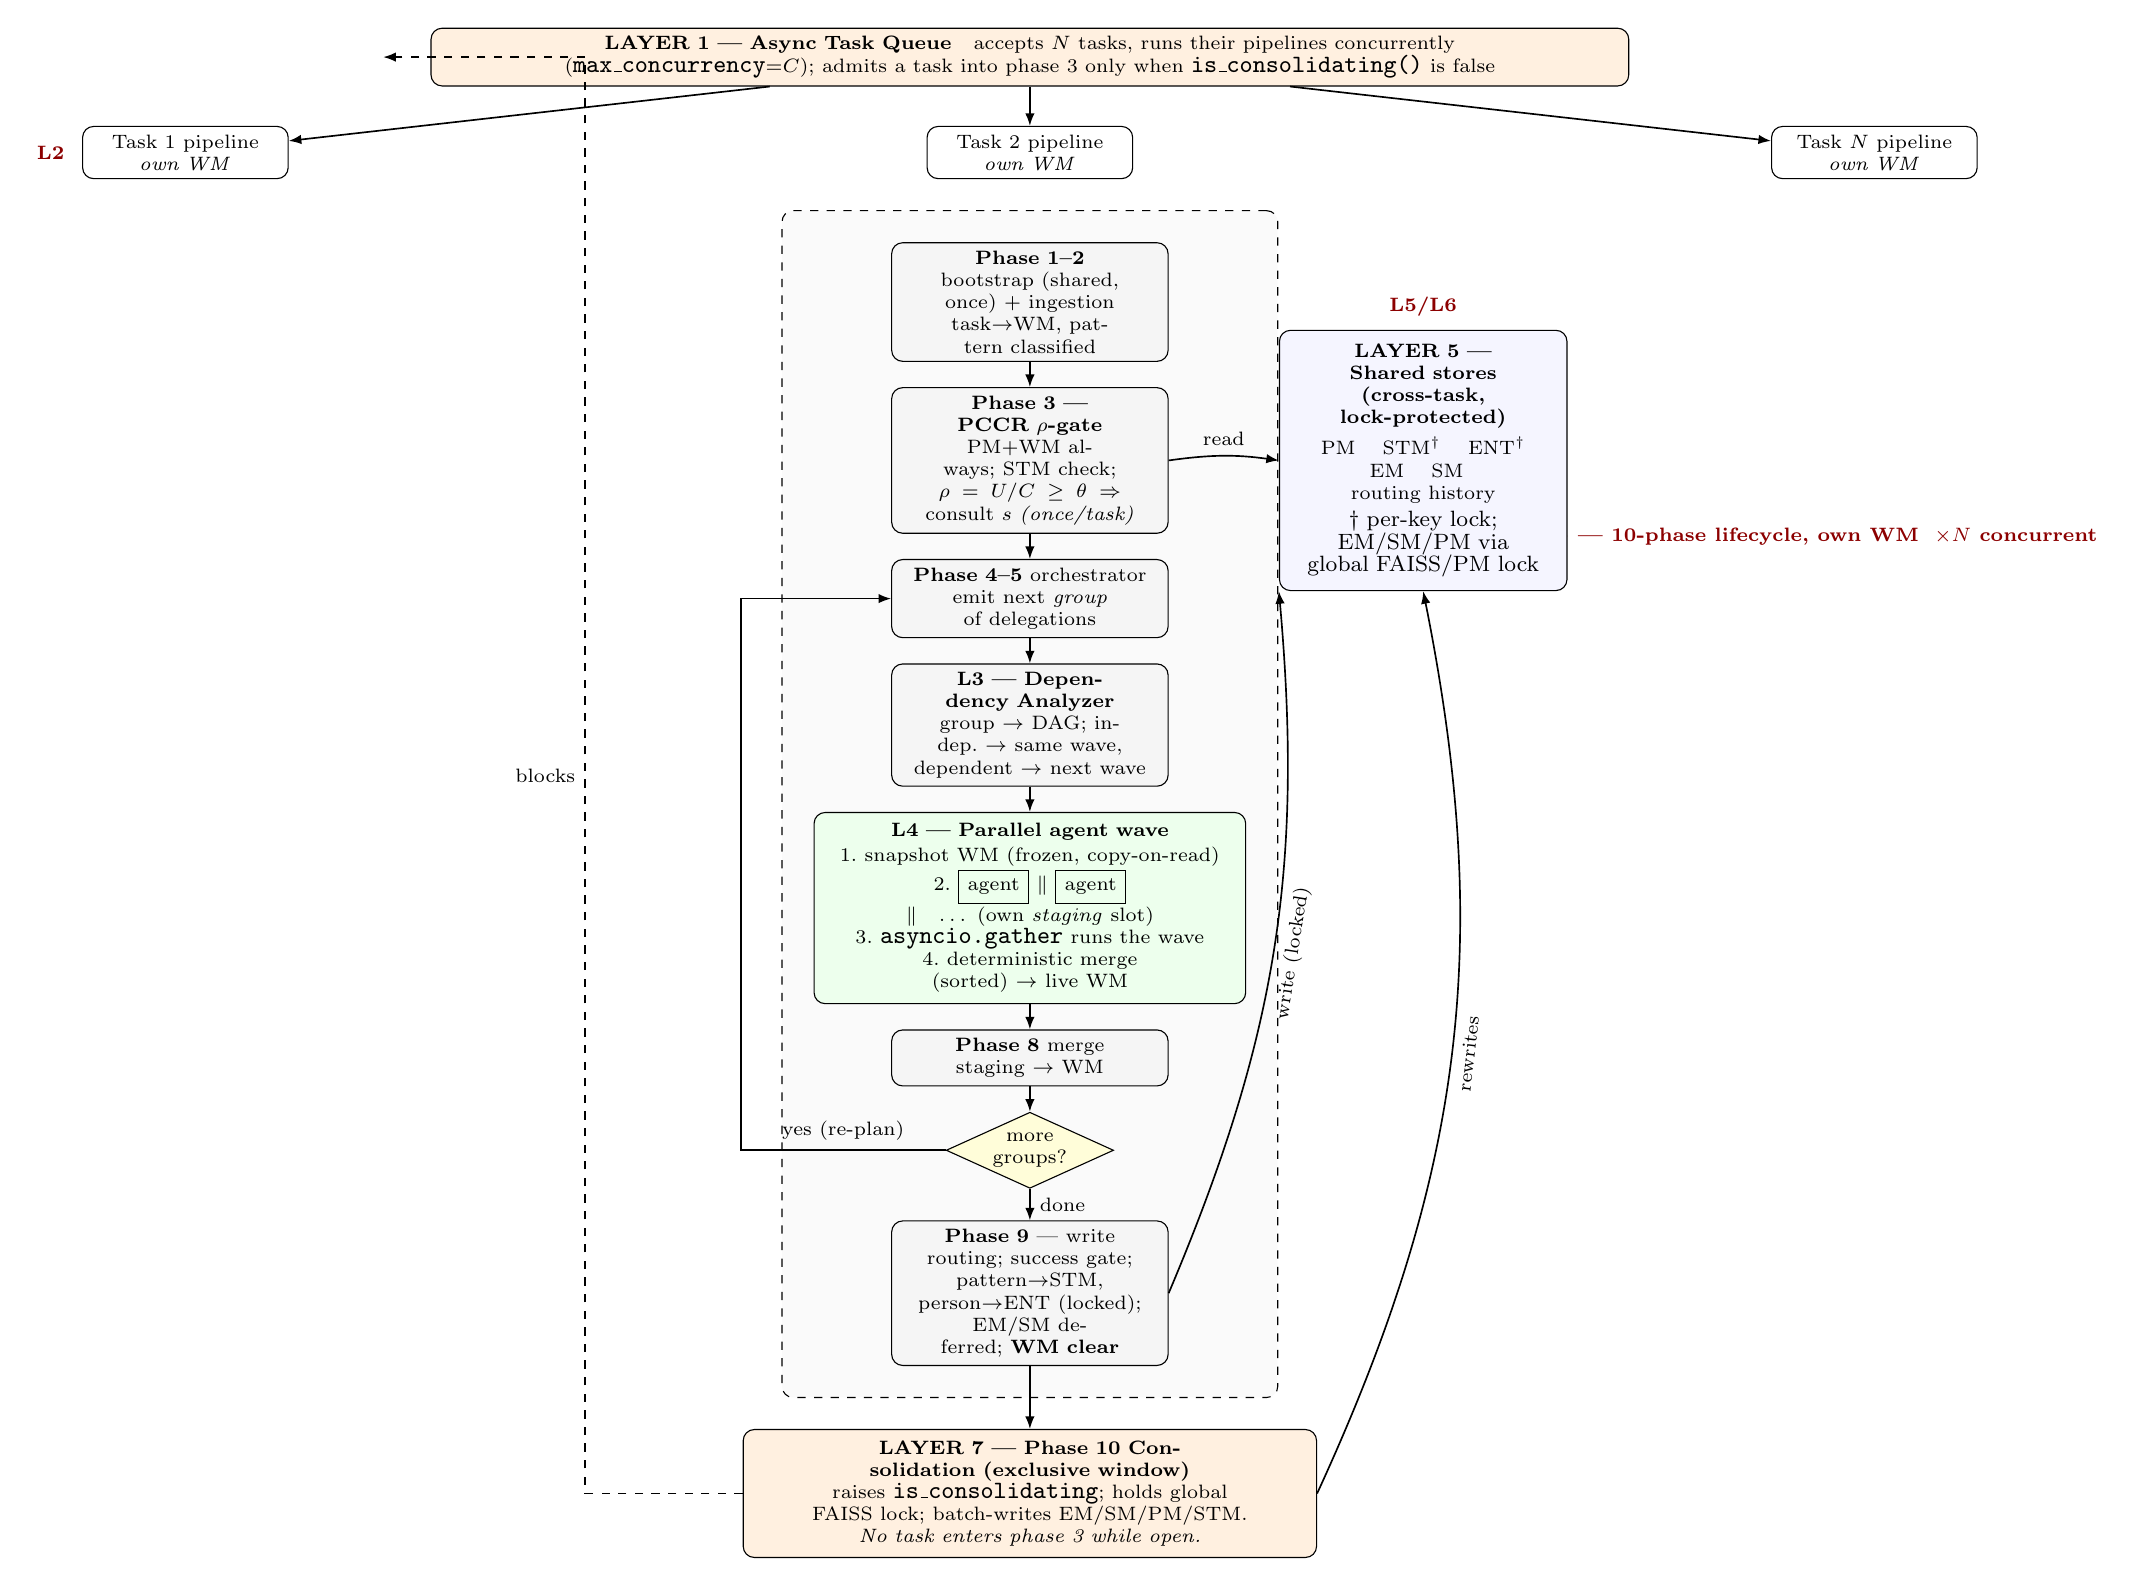
\begin{tikzpicture}[
  font=\scriptsize,
  box/.style   ={draw, rounded corners, align=center, inner sep=3pt, minimum height=6.5mm},
  phase/.style ={draw, fill=gray!8,  rounded corners, align=center, inner sep=3pt, minimum height=6.5mm, text width=33mm},
  group/.style ={draw, fill=green!7, rounded corners, align=center, inner sep=4pt, text width=52mm},
  storebox/.style={draw, fill=blue!4, rounded corners, align=center, inner sep=5pt, text width=33mm},
  cons/.style  ={draw, fill=orange!12, rounded corners, align=center, inner sep=4pt, text width=70mm},
  lyr/.style   ={font=\scriptsize\bfseries, text=red!55!black},
  arr/.style   ={-{Latex[length=1.6mm]}, semithick},
  darr/.style  ={-{Latex[length=1.6mm]}, dashed, semithick},
  node distance=3.2mm and 9mm
]
\node[box, fill=orange!12, text width=150mm] (queue)
  {\textbf{LAYER 1 — Async Task Queue}\quad accepts $N$ tasks, runs their pipelines concurrently
   (\code{max\_concurrency}=$C$); admits a task into phase 3 only when \code{is\_consolidating()} is false};
\node[box, below left=5mm and 18mm of queue, text width=24mm] (t1) {Task 1 pipeline\\\textit{own WM}};
\node[box, below=5mm of queue, text width=24mm]               (t2) {Task 2 pipeline\\\textit{own WM}};
\node[box, below right=5mm and 18mm of queue, text width=24mm](tn) {Task $N$ pipeline\\\textit{own WM}};
\node[lyr, left=1mm of t1] {L2};
\draw[arr] (queue) -- (t1); \draw[arr] (queue) -- (t2); \draw[arr] (queue) -- (tn);
\node[phase, below=8mm of t2] (p12) {\textbf{Phase 1--2}\\ bootstrap (shared, once) + ingestion\\ task$\to$WM, pattern classified};
\node[phase, below=of p12]    (p3)  {\textbf{Phase 3 — PCCR $\rho$-gate}\\ PM+WM always; STM check;\\ $\rho=U/C\ge\theta\Rightarrow$ consult $s$ \emph{(once/task)}};
\node[phase, below=of p3]     (p45) {\textbf{Phase 4--5} orchestrator\\ emit next \emph{group} of delegations};
\node[box, fill=gray!8, below=of p45, text width=33mm] (dag)
  {\textbf{L3 — Dependency Analyzer}\\ group $\to$ DAG; indep.\ $\to$ same wave,\\ dependent $\to$ next wave};
\node[group, below=of dag] (grp)
  {\textbf{L4 — Parallel agent wave}\\[1pt]
   1.\ snapshot WM (frozen, copy-on-read)\\
   2.\ \fbox{agent} $\parallel$ \fbox{agent} $\parallel\,\dots$ (own \emph{staging} slot)\\
   3.\ \code{asyncio.gather} runs the wave\\
   4.\ deterministic merge (sorted) $\to$ live WM};
\node[phase, below=of grp] (p8) {\textbf{Phase 8} merge staging $\to$ WM};
\node[draw, diamond, aspect=2.2, fill=yellow!15, below=of p8, inner sep=1pt, align=center] (dec) {more\\groups?};
\node[phase, below=4mm of dec] (p9)
  {\textbf{Phase 9} — write routing; success gate;\\ pattern$\to$STM, person$\to$ENT (locked);\\ EM/SM deferred; \textbf{WM clear}};
\draw[arr] (p12) -- (p3); \draw[arr] (p3) -- (p45); \draw[arr] (p45) -- (dag);
\draw[arr] (dag) -- (grp); \draw[arr] (grp) -- (p8); \draw[arr] (p8) -- (dec);
\draw[arr] (dec) -- node[right]{done} (p9);
\draw[arr] (dec.west) -- ++(-26mm,0) node[midway,above]{yes (re-plan)} |- (p45.west);
\begin{scope}[on background layer]
\node[draw, dashed, rounded corners, fill=black!2, fit=(p12)(p3)(p45)(dag)(grp)(p8)(dec)(p9),
      inner sep=4mm, label={[lyr]above right:{Per-task pipeline (Task $i$) — 10-phase lifecycle, own WM \;$\times N$ concurrent}}] (pipe) {};
\end{scope}
\node[storebox, right=14mm of p3, anchor=west] (stores)
  {\textbf{LAYER 5 — Shared stores}\\ \textbf{(cross-task, lock-protected)}\\[2pt]
   PM \;\; STM\textsuperscript{$\dagger$} \;\; ENT\textsuperscript{$\dagger$}\\
   EM \;\; SM \;\; routing history\\[2pt]
   \footnotesize $\dagger$ per-key lock; EM/SM/PM via global FAISS/PM lock};
\node[lyr, above=0.5mm of stores] {L5/L6};
\draw[arr] (p3.east) to[bend left=8] node[above,sloped]{read} (stores.west);
\draw[arr] (p9.east) to[bend right=14] node[below,sloped]{write (locked)} (stores.south west);
\node[cons, below=8mm of p9] (p10)
  {\textbf{LAYER 7 — Phase 10 Consolidation (exclusive window)}\\
   raises \code{is\_consolidating}; holds global FAISS lock; batch-writes EM/SM/PM/STM.\\
   \emph{No task enters phase 3 while open.}};
\draw[arr] (p9) -- (p10);
\draw[arr] (p10.east) to[bend right=18] node[below,sloped]{rewrites} (stores.south);
\draw[darr] (p10.west) -- ++(-20mm,0) |- node[near start,left]{blocks}([xshift=-6mm]queue.west);
\end{tikzpicture}%
}
\caption{The finalized \textbf{PCCR-2D} architecture at $N{=}4$. \textbf{Parallel tasks}
(L1--L2): the async queue runs $N$ pipelines concurrently, each with its own Working Memory but sharing
the locked cross-task stores. \textbf{Parallel sub-agents} (L3--L4): the orchestrator emits a group of
delegations, the dependency analyzer forms waves of independent sub-tasks, each wave runs against a
frozen WM snapshot and is merged back deterministically, and control re-plans until \textsc{finish}.
The $\rho$-gate (Phase~3) is unchanged and runs once per task before any parallelism.}
\label{fig:arch}
\end{figure*}

% =====================================================================
\section{Experiments}\label{sec:results}
% =====================================================================
\paragraph{Setup.} We evaluate on OfficeBench~\cite{officebench} with a \code{gpt-oss-120b} backbone
(served on Cerebras, temperature 0), which drives real Docker-sandboxed office applications. EM/SM are
FAISS \code{IndexFlatIP} over 384-d \code{all-MiniLM-L6-v2} embeddings. A task is correct only if all
its evaluation predicates pass. Baselines are \textbf{no-memory} and \textbf{retrieve-all} run through
the identical harness; all token counts are real \code{prompt+completion} usage.

\subsection{Routing efficiency (level-wise, held-out)}\label{sec:routing}
We first characterize the router level-by-level on held-out multi-agent splits---the 2-agent level
(calendar$+$email, 11 tasks) and 3-agent level ($+$document, 32 tasks)---sharing identical agents,
prompts, and consolidated memory, differing only in retrieval policy (Tables~\ref{tab:cmp}--\ref{tab:frontier}).
All methods reach identical accuracy; PCCR attains it at the lowest cost. The three-agent frontier has
a sharp knee: $\theta{:}1.0{\to}1.2$ cuts consultations $27{\to}6$ ($-78\%$) and injected tokens
$837{\to}96$ ($-89\%$) with \emph{no} accuracy loss. \textbf{At $\theta{=}1.2$ PCCR matches every
baseline's accuracy while issuing $\sim$87\% fewer consultations than retrieve-all (6 vs.\ 46) and
injecting $\sim$89\% fewer tokens.} Per-pattern consult rates match the $\rho$-model exactly: episodic
is pruned on pure lookups, entity where a profile is irrelevant, and both are consulted for
coordination---the aggregate saving is a sum of interpretable, store-specific decisions.

\begin{table}[t]
\centering\small
\setlength{\tabcolsep}{4pt}
\begin{tabular}{@{}llccc@{}}
\toprule
Level & Method & Acc & Consults & FAISS \\
\midrule
\multirow{2}{*}{2-agent (11)}
 & Retrieve-All & 5/11 & 20 & 27 \\
 & \textbf{PCCR} & 5/11 & \textbf{12} & \textbf{25} \\
\midrule
\multirow{2}{*}{3-agent (32)}
 & Retrieve-All & 10/32 & 46 & 72 \\
 & \textbf{PCCR} & \textbf{11/32} & \textbf{27} & \textbf{62} \\
\bottomrule
\end{tabular}
\caption{Held-out routing comparison ($\theta{=}1.0$). At equal accuracy PCCR cuts consultations
$\sim$41\% (2-agent) and $\sim$41\% (3-agent, $27$ vs.\ $46$); the $\theta$-sweep (Table~\ref{tab:frontier})
pushes this to $87\%$.}
\label{tab:cmp}
\end{table}

\begin{table}[t]
\centering\small
\begin{tabular}{@{}ccccc@{}}
\toprule
$\theta$ & Acc & Consults & FAISS & Inj.\ tokens \\
\midrule
1.0 & 11/32 & 27 & 60 & 837 \\
\textbf{1.2} & \textbf{11/32} & \textbf{6} & 38 & \textbf{96 ($-89\%$)} \\
1.4 & 8/32 & 6 & 37 & 96 \\
\bottomrule
\end{tabular}
\caption{Three-agent cost/quality frontier (self-consistent, shared memory). $\theta$ is a single
interpretable dial: a sharp knee at $1.2$ gives $-87\%$ consultations and $-89\%$ tokens at no
accuracy cost.}
\label{tab:frontier}
\end{table}

\subsection{Grounding the priors and a load-bearing test}\label{sec:grounding}
Two questions precede any full-scale claim: where do $C$ and $U$ come from, and is the benchmark even
memory-dependent? \textbf{Cost} is measured locally (the $30\times$ token-injection ratio above).
\textbf{Utility} is initialized counterfactually from a with/without-store ablation: for the
entity-critical pattern, ENT off $\to 0/8$, ENT on $\to 7/8$, giving $U(\text{ENT}){=}\mathbf{0.875}$.
For the \textbf{load-bearing} check we engineered a memory-critical set (8 episodic- $+$ 8
entity-critical tasks whose answer lives \emph{only} in a store): no-memory collapses to
$\mathbf{0/16}$ while PCCR reaches $\mathbf{16/16}$ (matching retrieve-all) at lower cost
($24$ vs.\ $32$ consults). This decisively answers the validity question---memory is used where
required, and PCCR routes to it.

\subsection{Full-scale accuracy by level and pattern}\label{sec:full}
Scaling to all 152 test tasks across nine applications and three difficulty levels (L1/L2/L3), the
fully-equipped router---confidence-gated routing, verified replay, a completion gate, a continual
short-term cache, and the fidelity mechanisms of \S\ref{sec:fidelity}---reaches
\textbf{parity} with retrieve-all ($0.474$ vs.\ $0.467$, within backbone run-to-run variance) while
the level and pattern breakdowns tell the substantive story (Tables~\ref{tab:cg-level}--\ref{tab:cg-pat}).

The \textbf{gate is protective}. On \textbf{L3}, indiscriminate retrieve-all \emph{collapses} to
$0.158$---below the no-memory floor of $0.228$---because injected episodes distract on long multi-step
tasks, whereas PCCR declines the unhelpful memory and tracks no-memory ($0.211$). On the
open-ended \code{multi\_app} pattern (78 of 152 tasks), na\"ive memory \emph{degrades} accuracy
($0.269 < 0.295$ no-memory); the fidelity mechanisms \emph{repair} this fully
($0.179{\to}0.244{\to}\mathbf{0.295}$), now matching no-memory and above retrieve-all. PCCR
simultaneously \emph{wins} on structured \code{doc\_process} ($0.680 > 0.600$) and rescues 8 tasks
both baselines miss. The honest headline: \emph{the gate mechanism is sound and protective; the
remaining overall gap is a systematic backbone weakness on open-ended tasks}, reproduced identically
across parallel and sequential full runs.

\begin{table}[t]
\centering\small
\setlength{\tabcolsep}{4pt}
\begin{tabular}{@{}lcccc@{}}
\toprule
Level & no-mem & retr-all & \textbf{PCCR} \\
\midrule
L1 (47) & $0.553$ & $\mathbf{0.723}$ & $0.681$ \\
L2 (48) & $0.500$ & $0.583$ & $\mathbf{0.583}$ \\
L3 (57) & $\mathbf{0.228}$ & $0.158$ & $0.211$ \\
\midrule
Total   & $0.414$ & $0.467$ & $\mathbf{0.474}$ \\
\bottomrule
\end{tabular}
\caption{Full-scale OfficeBench accuracy by difficulty level (152 tasks, \code{gpt-oss-120b},
$\theta_{\text{sim}}{=}0.45$). PCCR reaches \textbf{parity} overall and is \textbf{protective on L3},
where retrieve-all collapses \emph{below} no-memory.}
\label{tab:cg-level}
\end{table}

\begin{table}[t]
\centering\small
\setlength{\tabcolsep}{4pt}
\begin{tabular}{@{}lcccc@{}}
\toprule
Pattern & $n$ & no-mem & retr-all & \textbf{PCCR} \\
\midrule
data\_compute  & 10 & $0.700$ & $\mathbf{0.800}$ & $\mathbf{0.800}$ \\
doc\_process   & 25 & $0.480$ & $0.600$ & $\mathbf{0.680}$ \\
lookup         & 16 & $0.625$ & $\mathbf{0.812}$ & $0.688$ \\
multi\_app     & 78 & $0.295$ & $0.269$ & $\mathbf{0.295}$ \\
single\_action & 23 & $0.478$ & $\mathbf{0.609}$ & $0.565$ \\
\midrule
\textbf{Total} & 152 & $0.414$ & $0.467$ & $\mathbf{0.474}$ \\
\bottomrule
\end{tabular}
\caption{Accuracy by task pattern. PCCR repairs the \code{multi\_app} collapse
($0.179{\to}0.244{\to}\mathbf{0.295}$, now $>$ retrieve-all) and keeps the \code{doc\_process} win.}
\label{tab:cg-pat}
\end{table}

\subsection{Execution-fidelity mechanisms}\label{sec:fidelity}
With the backbone fixed, accuracy is gated not by \emph{which} store is consulted but by the
\emph{fidelity} of what the cascade injects and whether the agent may stop prematurely. Four
mechanisms---added without touching the $\rho$-gate or the ten phases---move OfficeBench from
$0.421$ to $0.474$. \textbf{(F1) Schema-validated injection}: episodic traces can contain invalid tool
calls; a sanitiser keeps only schema-valid \code{(app, action)} pairs on the EM$\to$prompt path, so
the agent never imitates a malformed call. \textbf{(F2) Inject-once scheduling}: the heavy procedural
block is injected only for the first $K{=}3$ steps, the light roadmap every step---cutting per-call
memory injection $5\times$ ($709{\to}146$ tokens). \textbf{(F3) Completion gate over both stop
signals}: the dominant multi-app failure is \emph{abandonment} (\code{got\_stuck} with outputs unmade),
so the gate intercepts both stop signals and re-prompts when a required output is missing---engagement
on the hard subset rose from ${\sim}9$ to $35$ of $64$ tasks. \textbf{(F4) Continual short-term cache}:
exercising the lifecycle's own success$\to$STM write \emph{during} evaluation (bounded, LFU/LRU, high
short-circuit threshold) lifts live STM hits $8{\to}12$, making genuine recurrences nearly free.

\subsection{The real-token reckoning}\label{sec:realtoken}
A central, easily missed finding: \emph{injected}-token savings do not imply \emph{real}-token savings
(Table~\ref{tab:realtoken}). Instrumenting true \code{usage} tokens across all arms under one $N{=}4$
harness, PCCR matches or slightly beats retrieve-all on accuracy ($72{=}72$ lean; $74{>}72$ improved)
yet costs \textbf{$30$--$60\%$ more real tokens}. The cause is \emph{call count}, not injection: the
completion gate's \code{got\_stuck} retries add $+38\%$ calls ($3146$ vs.\ $2284$), and every call
re-sends the dominant system$+$history bulk. Tellingly, the improved arm injects $12\%$ \emph{fewer}
memory tokens ($630$K vs.\ $712$K) yet costs $60\%$ \emph{more} real tokens---confirming injected
tokens is the wrong proxy for cost. The clean injected-token efficiency (\S\ref{sec:routing}, up to
$89\%$) is real and useful for context-window pressure, but on this agentic benchmark it does not
translate into a real-token win: PCCR buys its accuracy by doing more work, and the provider bills
that work. Reporting only injected tokens, as much prior work does, materially overstates savings.

\begin{table*}[t]
\centering\small
\setlength{\tabcolsep}{6pt}
\begin{tabular}{@{}lcccccc@{}}
\toprule
Arm & Accuracy & Real tokens & tok/call & LLM calls & Injected & STM hits \\
\midrule
no-memory (floor)        & $68/152$ & $\mathbf{3.35}$M & $\mathbf{1223}$ & $2743$ & $0$ & $0$ \\
retrieve-all (baseline)  & $72/152$ & $4.47$M & $1955$ & $\mathbf{2284}$ & $712$K & $0$ \\
lean PCCR                & $72/152$ & $5.82$M & $2342$ & $2484$ & $553$K & $13$ \\
improved PCCR            & $\mathbf{74/152}$ & $7.15$M & $2273$ & $3146$ & $\mathbf{630}$K & $10$ \\
\bottomrule
\end{tabular}
\caption{Real-token cost ledger ($N{=}4$, true prompt$+$completion usage). PCCR matches or beats
retrieve-all on accuracy but costs $30$--$60\%$ more \emph{real} tokens: the completion gate's retries
add $+38\%$ calls, and each call re-sends the system$+$history bulk. Improved injects $12\%$
\emph{fewer} memory tokens yet costs $60\%$ \emph{more} real tokens---injected-tokens is the wrong metric.}
\label{tab:realtoken}
\end{table*}

\subsection{Two-dimensional concurrency}\label{sec:parallel}
Because accuracy, calls, and injected tokens are all \emph{per-task}, they are identical whether the
schedule is sequential or parallel; concurrency touches only wall-clock time. We verify
\textbf{outcome equivalence} directly: over 60 tasks with per-task isolated environments the parallel
schedule produces \textbf{$60/60$ byte-identical} outcomes and identical final memory state
(invariants I1--I3). Under a deliberately \emph{shared} world, $2/60$ coordination tasks diverge only
on an incidental observation count while success, plan, and memory stay identical---exactly the single
divergence vector the correctness argument predicts, removed by isolation. Latency scales near-linearly
with concurrency up to the dependency critical path (Table~\ref{tab:scale}): at the measured backbone
latency ($0.516$\,s/call), $C{=}4$ is \textbf{$3.73\times$} faster (up to $13.5\times$ at $C{=}16$),
and $100$ tasks finish in $61.1$\,s versus $227.7$\,s sequential.

\begin{table}[t]
\centering\small
\setlength{\tabcolsep}{4.5pt}
\begin{tabular}{@{}lccccc@{}}
\toprule
$C$ & 1 & 2 & 4 & 8 & 16\\
\midrule
Speedup        & $0.96\times$ & $1.89\times$ & $\mathbf{3.73\times}$ & $7.15\times$ & $13.47\times$\\
Wall-clock cut & $-5\%$ & $47\%$ & $73\%$ & $86\%$ & $93\%$\\
\bottomrule
\end{tabular}
\caption{Speedup vs.\ task-concurrency $C$ (100 tasks, $L{=}0.516$\,s/call). The win is dominated by
parallel tasks; parallel sub-agents are a secondary benefit on coordination tasks.}
\label{tab:scale}
\end{table}

\subsection{PCCR-2D: the full architecture}\label{sec:twod}
Our finalized architecture, \textbf{PCCR-2D} (Fig.~\ref{fig:arch}), runs the complete pipeline: the
PCCR router feeding a general DAG re-plan orchestrator whose parallel, memory-backed sub-agents realize
the second concurrency dimension at $N{=}4$. We report its result exactly as measured:
\textbf{$65/152$ at $4.9$M real tokens}, $36.2$ min wall-clock (Table~\ref{tab:final}). This is the
system the abstract and Fig.~\ref{fig:arch} promise, and we neither inflate nor bury it: it is
efficient and fast, but its accuracy is \emph{capped by the orchestrator}, not by the memory.

We establish this by controlled comparison. \textbf{Replacing} the router entirely with pure
decomposition (\emph{2D-only}) collapses accuracy to $18/152$ (L3 $1/57$): only $\sim$5\% of tasks are
genuinely parallelizable fan-outs; the rest are sequential pipelines that decomposition shreds by
discarding whole-task context. \textbf{Layering} a targeted, deterministic fan-out fast-path on top of
the intact router (\emph{PCCR-2D fan-out}) preserves accuracy ($68$) and is strictly additive---it
solves $+2$ tasks 1D misses with \emph{zero} regressions, and on its niche wins $4/4$ vs.\ 1D's $3/4$
at $3.3\times$ fewer tokens. The \textbf{fully general} orchestrator of PCCR-2D, driven from an
initial $8.1$M tokens down to $4.9$M via inject-once, a round cap ($8{\to}4$), and plan-then-execute
batching, plateaus at $65$---below both the flat router ($73$) and the targeted layer ($68$). The
bottleneck is the orchestrator's decomposition quality: it re-plans one group at a time and mis-splits
dependent chains, losing the coherence a single agent keeps in context, which no cost trick fixes.
The lesson is precise: within this architecture, \emph{concurrency is a latency and cost tool, not an
accuracy tool}. Accuracy comes from the memory router; the two-dimensional schedule makes it fast and
optimizes its token budget; general task decomposition is a niche win (clean fan-outs), not a general
one. We present PCCR-2D's $65@4.9$M honestly on that basis.

\begin{table*}[t]
\centering\small
\setlength{\tabcolsep}{8pt}
\renewcommand{\arraystretch}{1.15}
\begin{tabular}{@{}llcccccc@{}}
\toprule
Arm & Exec & Accuracy & Real tokens & tok/call & Calls & Injected & Wall (min) \\
\midrule
no-memory              & seq          & $66$ & $\mathbf{3.38}$M & $1628$ & $\mathbf{2075}$ & $0$    & $58.4$ \\
retrieve-all           & seq          & $\mathbf{76}$ & $5.02$M & $2161$ & $2323$ & $778$K & $70.6$ \\
PCCR (router$+$PERF)   & \textbf{par} & $73$ & $6.87$M & $\mathbf{1810}$ & $3796$ & $641$K & $\mathbf{26.6}$ \\
\midrule
PCCR-2D (fan-out)      & par          & $68$ & $5.55$M & $1340$ & $4140$ & $609$K & $22.3$ \\
\textbf{PCCR-2D (full)}& par          & $65$ & $\mathbf{4.90}$M & $1908$ & $2568$ & $471$K & $36.2$ \\
\bottomrule
\end{tabular}
\caption{Final head-to-head, full-152, \code{gpt-oss-120b}. Sequential baselines (no parallel
architecture---that is our contribution) vs.\ PCCR on its parallel schedule ($N{=}4$). Real tokens $=$
prompt$+$completion; Wall $=$ wall-clock minutes. \textbf{Top block:} the PCCR router matches
retrieve-all accuracy within backbone noise ($73$ vs.\ $76$) and finishes $2.7\times$ faster, but---
because real cost is driven by call count---costs more \emph{real} tokens (\S\ref{sec:realtoken});
it wins on tok/call and injected tokens. \textbf{Bottom block (second dimension):} \emph{PCCR-2D
(fan-out)} layers a targeted fast-path and preserves accuracy ($68$, additive); \textbf{PCCR-2D (full)},
our finalized architecture with the general DAG re-plan orchestrator (Fig.~\ref{fig:arch}), lands at
\textbf{$65$ at $4.9$M real tokens}---efficient and fast, but accuracy-capped by the orchestrator below
the flat router. (Replacing the router outright with pure decomposition, \emph{2D-only}, collapses
accuracy to $18$; \S\ref{sec:twod}.)}
\label{tab:final}
\end{table*}

\subsection{Generalisation: LongMemEval}\label{sec:lme}
To test the router on a benchmark \emph{designed} for memory we add
LongMemEval~\cite{longmemeval} (multi-session chat histories), whose abilities map onto our stores.
On $90$ balanced retrieval questions, at equal cost PCCR matches Boolean session-recall ($0.735$) while
halving the expensive turn-level SM searches ($90{\to}45$); on $30$ end-to-end QA questions PCCR and
retrieve-all reach the \emph{same} accuracy ($0.733$) with PCCR at $-17\%$ consults and half the
turn-level searches. Parallel execution is outcome-identical to sequential here too. Where memory
\emph{helps}, the gate \emph{consults}; where it does not (\S\ref{sec:full}, L3), it \emph{declines}
---the adaptive thesis in full.

% =====================================================================
\section{Discussion and Limitations}
% =====================================================================
Our results delineate what does and does not transfer. The $\rho$-gate router is a robust,
benchmark-agnostic contribution: it reduces consultations and injected tokens substantially at no
accuracy cost, protects accuracy where indiscriminate retrieval is harmful, and is governed by one
interpretable dial. The concurrency architecture is a clean systems contribution with a proven
equivalence guarantee. Three honest caveats temper the story. \textbf{First}, injected-token efficiency
is not real-token efficiency; a memory method's true cost is dominated by call count, and we encourage
the community to report real usage. \textbf{Second}, general task decomposition, despite being an
appealing architectural idea, does not by itself raise accuracy---a good flat memory agent is a strong
baseline that decomposition struggles to beat. \textbf{Third}, the residual full-scale gap is a
systematic backbone weakness (malformed-action loops on open-ended \code{multi\_app} tasks under
\code{gpt-oss-120b}), reproduced identically across parallel and sequential runs. Limitations include
single-backbone evaluation, run-to-run stochasticity, and a coarse keyword-based dependency analyzer; a
multi-seed, multi-backbone study with variance reporting and a learned/semantic dependency analyzer are
the natural next steps.

% =====================================================================
\section{Conclusion}
% =====================================================================
We presented \textbf{PCCR-2D}, a phase-conditioned, cost-gated memory router for multi-agent LLM
systems extended with two dimensions of concurrency. Its router cuts store consultations by
$41$--$87\%$ and injected tokens by up to $89\%$ at equal accuracy, reaches full-scale parity with
retrieve-all while protecting accuracy where indiscriminate retrieval collapses, and runs
$2.2$--$2.7\times$ faster in wall-clock with provably identical outcomes ($60/60$ byte-identical). The
full architecture achieves $65/152$ at $4.9$M real tokens---which we report honestly: it is efficient
and fast, but accuracy-capped by the DAG re-plan orchestrator rather than by the memory. We paired
these results with a candid correction---injected-token savings do not imply real-token savings---and a
scoping analysis that locates the benefit in the router and schedule rather than in general task
decomposition. ``Which memory to consult'' should be a tunable, phase-aware, cost-sensitive decision
rather than a reflex, and ``how to execute'' a concurrency question answerable without disturbing it.

\begin{thebibliography}{99}\small
\setlength{\itemsep}{1pt}
\bibitem{coala} T.~Sumers et al. Cognitive Architectures for Language Agents (CoALA). TMLR, 2024.
\bibitem{survey1} Memory for Autonomous LLM Agents: Mechanisms, Evaluation, and Emerging Frontiers. arXiv, 2026.
\bibitem{survey2} Anatomy of Agentic Memory: Taxonomy and Empirical Analysis. arXiv, 2026.
\bibitem{pocket} M.~Gaikwad. Did You Check the Right Pocket? Cost-Sensitive Store Routing for Memory-Augmented Agents. ICLR Workshop, 2026.
\bibitem{budgetmem} H.~Zhang et al. Learning Query-Aware Budget-Tier Routing for Runtime Agent Memory (BudgetMem). arXiv, 2026.
\bibitem{memrouter} MemRouter: Memory-as-Embedding Routing for Long-Term Conversational Agents. arXiv, 2026.
\bibitem{umem} Towards Autonomous Memory Agents (U-Mem). arXiv, 2026.
\bibitem{agemem} Agentic Memory: Learning Unified Long-Term and Short-Term Memory Management for LLM Agents. arXiv, 2026.
\bibitem{fluxmem} Choosing How to Remember: Adaptive Memory Structures for LLM Agents (FluxMem). arXiv, 2026.
\bibitem{legomem} LEGOMem: Modular Procedural Memory for Multi-agent LLM Systems. arXiv:2510.04851, 2025.
\bibitem{mirix} Y.~Wang, X.~Chen. MIRIX: Multi-Agent Memory System for LLM-Based Agents. arXiv:2507.07957, 2025.
\bibitem{rcr} RCR-Router: Efficient Role-Aware Context Routing for Multi-Agent LLM Systems. arXiv:2508.04903, 2025.
\bibitem{amem} A-MEM: Agentic Memory for LLM Agents. NeurIPS, 2025.
\bibitem{memgpt} C.~Packer et al. MemGPT: Towards LLMs as Operating Systems. arXiv:2310.08560, 2023.
\bibitem{mem0} Mem0: Building Production-Ready AI Agents with Scalable Long-Term Memory. 2025.
\bibitem{memos} MemOS: An Operating System for Memory-Augmented Generation. EMNLP, 2025.
\bibitem{voi} R.~Howard. Information Value Theory. IEEE Trans. SSC, 1966.
\bibitem{meta} S.~Russell, E.~Wefald. Principles of Metareasoning. Artificial Intelligence, 1991.
\bibitem{dyntaskmas} DynTaskMAS: A Dynamic Task-Graph Multi-Agent System with Asynchronous Parallel Execution. arXiv:2503.07675, 2025.
\bibitem{gap} GAP: Graph-based Agent Planning with Dependency-Aware Parallelism. arXiv:2510.25320, 2025.
\bibitem{spoq} SPOQ: Scheduling Parallel Orchestration via Topological Wave Dispatch. arXiv, 2026.
\bibitem{adaptorch} AdaptOrch: Adaptive Parallel/Sequential Orchestration for LLM Agents. arXiv, 2026.
\bibitem{officebench} T.~Wang et al. OfficeBench: Benchmarking Language Agents across Multiple Applications for Office Automation. arXiv:2407.19056, 2024.
\bibitem{longmemeval} D.~Wu et al. LongMemEval: Benchmarking Chat Assistants on Long-Term Interactive Memory. ICLR, 2025.
\end{thebibliography}

\end{document}
